\chapter{Binary Analysis}
Binary analysis is a task that requires mastering a multitude of tools and techniques. Some of them are fairly trivial
to use while others require more effort. The following sections outline the techniques used in binary analysis and the
relevant tools.



\section{Preliminary Operations}
The following provides a checklist of operations that might be needed when analysing a binary; it is not meant to be a
compulsory list and it is by no means exhaustive, but it provides an idea of the minimal operations to be carried out.


\subsection{File Identification}
The first step is to identify the file and its nature. This can be done by means of several programs:
\begin{enumerate}
    \item {\ttfamily file} utility for the identification of a file that does not rely on extension info, but actually
        scans the binary in search for known headers and patterns;
    \item {\ttfamily binwalk} analyses images for embedded code and files inside firmware images;
    \item {\ttfamily xxd} dumps the content of a file in hex format while showing the offset, the value and the ASCII
        representation of each byte in the file;
    \item {\ttfamily objdump} dumps the content of a binary and allows for the interpretation of file headers, sections
        and instructions (if dealing with an ELF);
    \item {\ttfamily strings} prints out all of the strings of a binary;
    \item {\ttfamily readelf} provides a handy tool to navigate and explore an ELF;
    \item {\ttfamily nm} helps to read symbols and demangle function names.
\end{enumerate}


\subsection{Dependencies, Function and System Calls}
After identifying the file it is important to understand what kind of dependencies the program has and which functions
are invoked in execution; most of the existing tools will track the program execution in order to provide the
information required \footnote{When analysing malware or untrusted code avoid running code in the base system and always
try to use sandboxed environments}. Some of the tools used to this aim are:
\begin{enumerate}
    \item {\ttfamily ldd} which examinates the dependencies of an ELF file (if a dependency is resolved and satisfied
        the program will print the location of the shared object file and its memory mapping or "{\ttfamily not found}"
        otherwise);
    \item {\ttfamily ltrace} runs the program and intercepts dynamic library calls and signals received by the process;
    \item {\ttfamily strace} runs the program and intercepts system calls and signals received by the process;
\end{enumerate}



\section{Disassembly}
Disassembly is the operation of translating the code contained in binaries into human readable instructions. Normally
this operation can be carried out by means of:
\begin{itemize}
    \item Static Disassembly which involves the extraction of instructions from a binary without executing it. This
        consists mainly of two renown techniques:
        \subitem Linear Disassembly which is not control flow sensitive as it iterates through the code segments and
        decode all of the bytes into a list of sequential instructions;
        \subitem Recursive Traversal which is control flow sensitive that follows jumps and calls to discover code;
    \item Dynamic Disassembly (also called execution tracing) that logs instructions as the are executed.
\end{itemize}
The entire operation takes place in 3 steps:
\begin{enumerate}
    \item Load the binary;
    \item Find the machine instructions;
    \item Translate them into intelligible mnemonic.
\end{enumerate}
The second step is the most difficult as it is error prone and often hindered by obfuscation techniques which will be
discussed at later stage.


\subsection{Static Disassembly}

\subsubsection{Linear Disassembly}
As already mentioned above, linear disassembly iterates through all of the code segments and parses all of the bytes
encountered into instructions. The main disadvantage of linear disassemblers is related to the fact that some bytes
might be interpreted as instructions even when they are not - e.g. Visual Studio intersperses jump tables with code
without referencing exactly where that data might be; thus inline data might be parsed as an invalid opcode or even
worse as valid but meaningless instructions (this is quite likely on very dense ISA's as the x86).
Additionally, when dealing with variable length ISA's, the disassembler might desynch with respect to the effective
instruction stream; typically the disassembler will synch again with the execution flow, but this might induce the
misinterpretation or the complete loss of the very first instructions following inline data.V

\subsubsection{Recursive Disassembly}
In order to obviate to the issues of linear disassembly, recursive techniques rely on function calls and jumps for code
discovery; this allows to work around the presence of inline data when disassemblying. However, as control flows might
be articulated and difficult to follow, recursive disassemblers might lose entire blocks of code entirely.


\subsection{Dynamic Disassembly}

\subsubsection{Tracing}
Tracing is the ability to extract instructions from the binary as it gets executed. At a very low level this is done by
means of the {\ttfamily ptrace/wait} framework. \footnote{The {\ttfamily wait} instruction \textit{waits} for a state
change (terminated, stopped/resumed by signals) in the child process. If the instruction in not issued on a terminated
child this will become a zombie as there will be no parent process to clear it up}. The {\ttfamily ptrace} instruction
provides means for a parent process, calledv\textit{tracer}, to observe and control the execution of a child process,
the \textit{tracee}, by investigating its memory and registers. A tracee first needs to be attached to a tracer;
attachment works on a "per thread" basis. After a successful attachment data can be inspected by means of {\ttfamily
PTRACE\_PEEK*} requests that will return 0 in case of success or -1 otherwise (with appropriate {\ttfamily errno}). The
tracing typically commences with either:
\begin{itemize}
    \item the parent calling {\ttfamily fork} and having the child calling {\ttfamily PTRACE\_TRACEME}. This call is the
        only one done by the tracee and shall not be used if the parent is not expecting to trace the child;
    \item the parent calling {\ttfamily ptrace} with one of the two following options:
        \subitem {\ttfamily PTRACE\_ATTACH} which sends a {\ttfamily SIGSTOP} to the tracee;
        \subitem {\ttfamily PTRACE\_SEIZE} which does not stop the tracee.
\end{itemize}
When traced, the child will stop at each signal (even if ignored), with the only exception of the {\ttfamily SIGKILL}.
The attachment is concluded with a {\ttfamily PTRACE\_DETACH}. After stopping execution, this can be resumed by calling
the {\ttfamily PTRACE\_CONT}; if data is non-zero it is interpreted as the number of the signal to be delivered to the
tracee. The calls to {\ttfamily PTRACE\_SYSCALL} and {\ttfamily PTRACE\_SINGLESTEP} respectively stop the tracee with a
{\ttfamily SIGTRAP} at the entry/exit of a system call or at the execution of the next instruction. The calls to
{\ttfamily PTRACE\_SYSEMU} and {\ttfamily PTRACE\_SYSEMU\_SINGLESTEP} continue to stop on entry of a system call or the
next instruction for the latter. {\ttfamily PTRACE\_PEEKTEXT} and {\ttfamily PTRACE\_PEEKDATA} read a word at a specific
address of the tracee's memory (these two are equivalent requests under linux as there is no segregation between text
and data). {\ttfamily PTRACE\_PEEKUSER} allows for the investigation of the tracee's user area. The {\ttfamily
PTRACE\_GETREGS}, {\ttfamily PTRACE\_GETFPREGS} and {\ttfamily PTRACE\_GETREGSET} can copy, respectively, the general
purpose registers, the floating point registers or the vector registers to a specific address.

\subsubsection{Debuggers}
All of the techniques described above can be quite cumbersome when used in a productive environment; luckily most of the
debuggers take care of the low level work for the user. One of the most famous debuggers is \textbf{GDB}; it offers:
\begin{itemize}
    \item \textit{breakpoints} that interrupt execution when a certain instruction has been reached;
    \item \textit{watchpoints} that interrupt execution when a certain variable has been changed;
    \item \textit{catchpoints} that interrupt the program when an exception is thrown or a library is called.
\end{itemize}
These can be implemented in hardware (in a limited number with {\ttfamily rwx} permission) or software (unlimited number
with {\ttfamily --x} permissions).

\paragraph{Software Breakpoints}
When a breakpoint is found at address $\alpha$ the execution is arrested with the instruction {\ttfamily INT3 [0xCC]}
which launches a {\ttfamily SIGTRAP} intercepted by the debugger tracing the execution. {\ttfamily PTRACE\_PEEKTEXT} is
used to save the content of address $\alpha$ and the instruction is here replaced with {\ttfamily INT3} by means of
{\ttfamily PTRACE\_POKETEXT}. The instructions {\ttfamily PTRACE\_CONT} and {\ttfamily wait/waitpid} are used for the
next {\ttfamily SIGTRAP}. The instructions {\ttfamily PTRACE\_GETREG} and {\ttfamily PTRACE\_SETREG} are used to
inspect the program execution and manipulate it.

\paragraph{DWARF}
The DWARF is a debugging standard that establishes a default format for data representation: the Debugging Information
Entry (DIE). Each DIE has a tag and different attributes. A DIE can have others nested for children and refer to other
DIEs in tree fashion. The format uses two tables:
\begin{itemize}
    \item Line Number Table mapping code locations to source code lines and specifies which instructions are part of the
        prologue of a function ({\ttfamily .debug\_line});
    \item Call Frame Information Table allows debuggers to locate frames on the call stack.
\end{itemize}

\subsubsection{Code Coverage}
Unfortunately the use of tracing techniques might not be suitable when exploring binaries with large portions of code
seldomly executed.
In order to improve code coverage additional techniques might be used such as:
\begin{itemize}
    \item Testing with make (Makefile);
    \item Fuzzing (generation/mutation based fuzzers);
    \item Symbolic Execution.
\end{itemize}
All of the above mentioned techniques will be described separately within the present document.



\section{Analysing Control and Data Flows}
When code is disassembled it might be in such a form that makes it really difficult to be managed, especially when
dealing with stripped binaries. Modern disassemblers will try to:
\begin{itemize}
    \item \textit{Compartmentalise} the code into basic blocks - i.e. chunks of code containing jumps or return
        instructions only at the end - logically connected to each other;
    \item \textit{Reveal Control Flow} by tracking control transfer between code block
\end{itemize}


\subsection{Functions Detection}
Functions are the basic blocks used by high level languages to group a sequence of logically connected instructions;
their detection makes binary code a lot easier to handle and understand. For binaries compiled with their symbolic
information this is very trivial to do as the symbol table ({\ttfamily SYMTAB}) specifies the set of functions along
with their names. For stripped and optimised binaries this is way harder; the source level information are meaningless
as pieces of code might be scattered throughout the code section or even shared (overlapping code blocks). The
predominant strategy for function detection is the use of \textit{function signature} which are code patterns typically
found at the beginning and the end of functions. Signature based detection normally starts by locating the code
addressed by a {\ttfamily call} instruction; this technique is sufficiently accurate, and allows function detection also
in presence of indirect or tail \footnote{A tail call happens when a function terminates with a call to another
function; normally the compiler optimises tail calls by removing the ret instruction and using a jump} calls. This
because function signature databases normally contains instruction patterns for well known prologues and epilogues.
Another techniques that could help in circumventing the function detection problem entirely relies on the
{\ttfamily .eh\_frame} section which contains DWARF based debugging features. This technique requires stack unwinding.

\subsubsection{Stack Unwinding}
The {\ttfamily .eh\_frame} is basically a large table that, for each machine instruction, specifies how to compute where
the return address and the callee saved registers are stored. The rows correspond to machine instructions while the
columns represent the registers and the return address. Each cell of the table holds a rule detailing how the contents
of the register or the return address will be restored for the previous stack frame. These can be complex expressions,
but are normally expressed in terms of registers, constants and the Canonical Frame Address ({\ttfamily CFA} an
invariant of the execution that normally corresponds to the value in {\ttfamily rsp} before the function call. Each row
of the table must cover a range of instructions from its address to the one of the row below and if constructed in its
entirety would be unmanageable and larger than the progrsm itself; the DWARF standard obviates to the problem by
encodyng the table by using a compact bytecode that is only executed on demand to build the unwind table. The bytecode
defines the rows of the table by expressing the offset with the previous line; this means that all of the table can be
represented in a compact way, but in order to reach a certain location within it must run all of the bytecode
instructions (which might render the entire unwinding process painfully slow).

\subsubsection{Object Oriented Code}
Executables developed in object oriented languages, like C++, present additional hurdles to reverse engineers; in fact
exception handling and inheritance increment code complexity to a level where code is substantially more difficult to
understand. In particular, the latter is implemented by means of a specific data structure called \textit{vtable} which
is used by classes' function pointers (\textit{vptr}) to determine which function must be called in case of overloading
and inheritance.


\subsection{Control-Flow Graph}
A control flow graph provides a convenient representation of the code of a binary; instructions enclosed within
branching instructions (\textit{jump} and \textit{call}) represent a basic block which is defined as a set of
instructions with a single entry point at the beginning and one exit point at the end. Basic blocks are the nodes of the
CFG and are connected each other by branching edges; when branch edges jump back to a code block previously explored
there is a potential loop. The CFG is normally built for a single function and therefore call branches are not included
as they point towards code that is outside of the function itself. Figure \ref{CFG} shows an example of CFG.

\begin{figure}[!htbp]
    \begin{center}
        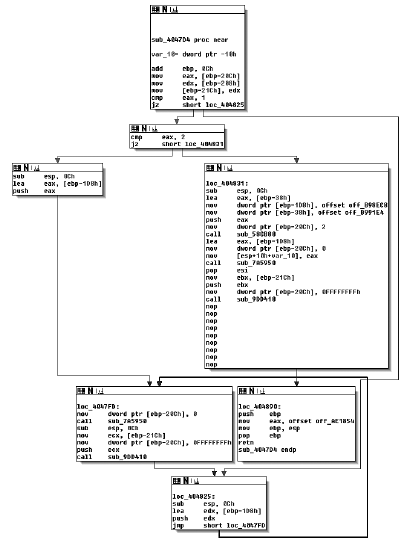
\includegraphics{./pics/CFG.png}
        \caption{Control-Flow Graph}
        \label{CFG}
    \end{center}
\end{figure}


\subsection{Call Graph}
A call graph represents relationships between functions; each functions is a node and each call is a link (recursive
calls are represented by a loop). A static call graph represents a graph of all of the possible execution call paths,
while a dynamic call graph is built at runtime by a profiler. Building a static call graph is an overapproximation
because:
\begin{itemize}
    \item when function pointers or virtual methods are invoked, a combination of dataflow and data type analysis could
        limit the set of potential targets;
    \item if a program loads code dynamically there might be a problem of code coverage.
\end{itemize}

